\documentclass{article}
\usepackage{tikz}
\usetikzlibrary{positioning, shapes.geometric, arrows.meta}

\begin{document}

\begin{figure}[h]
    \centering
    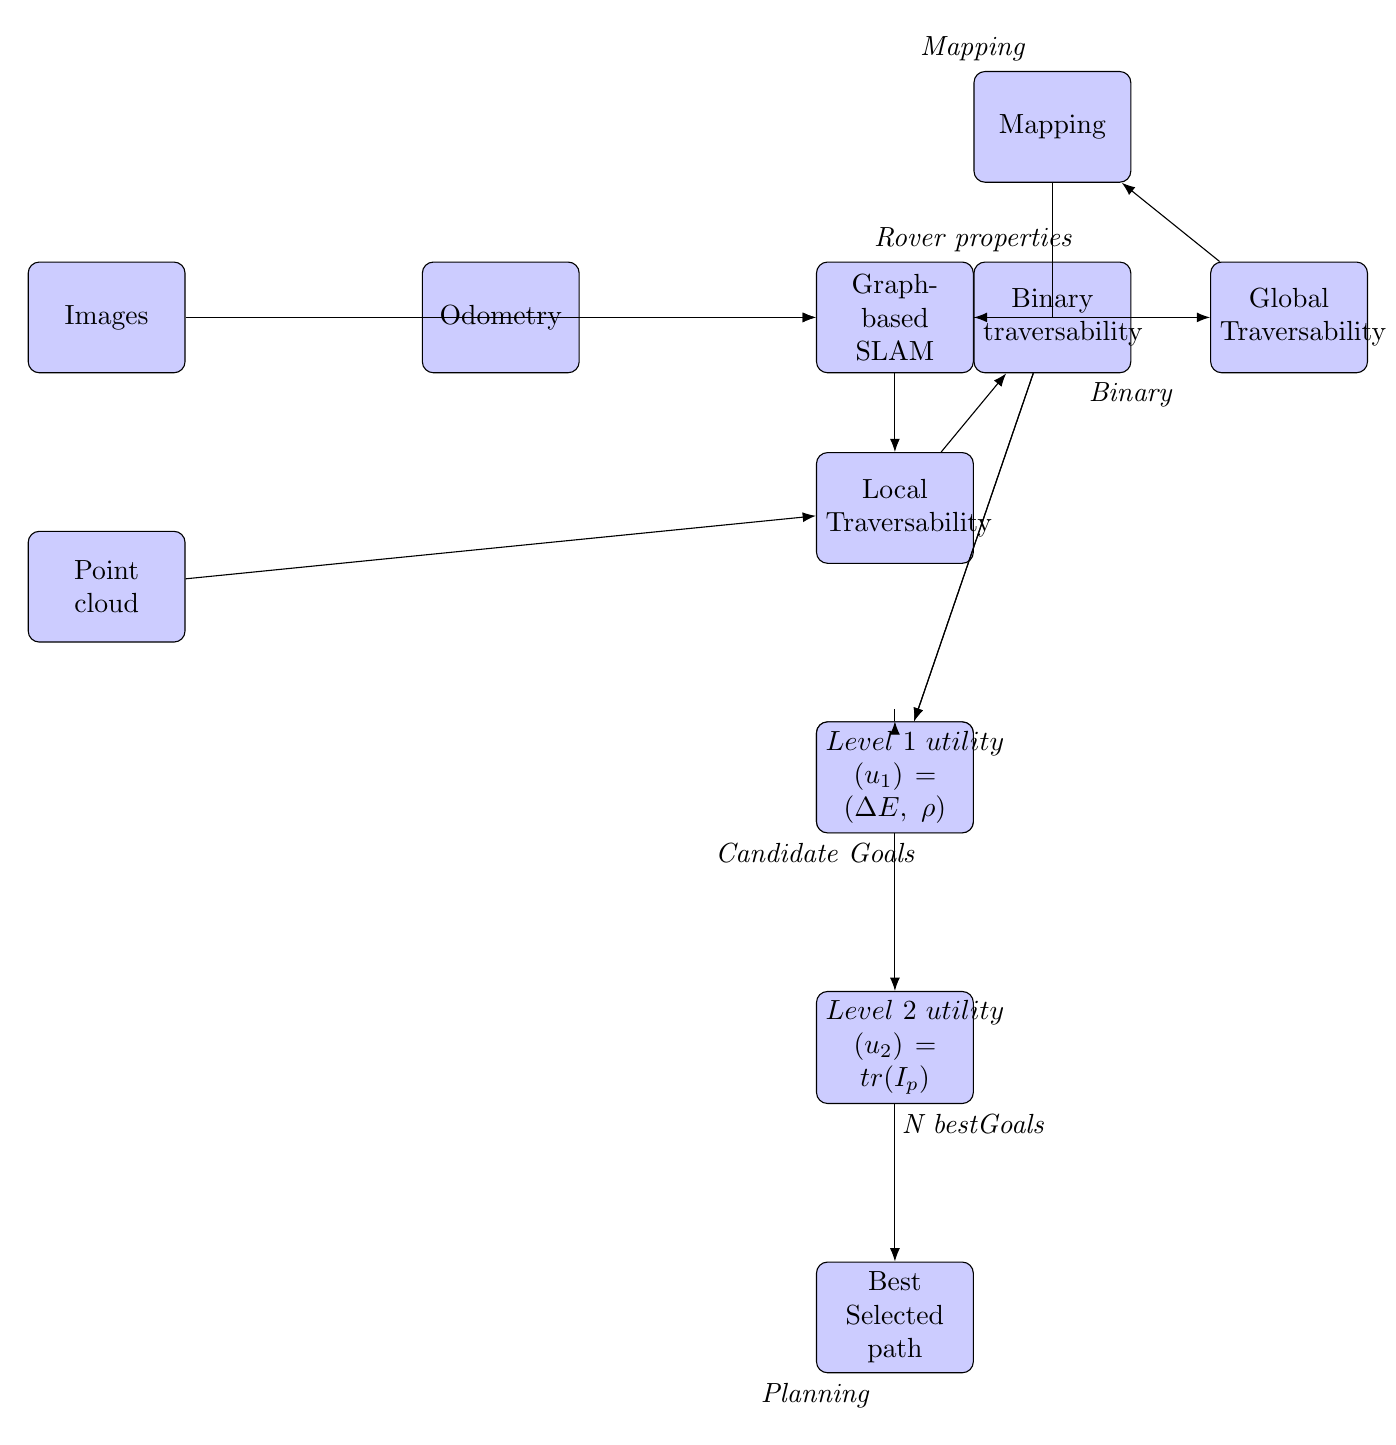
\begin{tikzpicture}[node distance=1cm, auto, >=Latex]
        % Define styles
        \tikzstyle{block} = [rectangle, draw, fill=blue!20, text width=5em, text centered, rounded corners, minimum height=4em]
        \tikzstyle{line} = [draw, -Latex]

        % Nodes
        \node [block] (graph) {Graph-based \\ SLAM};
        \node [block, below=of graph] (local) {Local \\ Traversability};
        \node [block, right=of graph, xshift=2cm] (global) {Global \\ Traversability};
        \node [block, below=of local, yshift=-1cm] (frontier) {Frontier detection};
        \node [block, left=of graph, xshift=-2cm] (odometry) {Odometry};
        \node [block, left=of odometry, xshift=-2cm] (images) {Images};
        \node [block, below=of images, yshift=-1cm] (pointcloud) {Point cloud};
        \node [block, below=of local, yshift=-1cm] (utility1) {$Level~1~utility$ \\ $(u_1)=(\Delta E,~\rho)$};
        \node [block, below=of utility1, yshift=-1cm] (utility2) {$Level~2~utility$ \\ $(u_2)=tr(I_p)$};
        \node [block, below=of utility2, yshift=-1cm] (bestpath) {Best \\ Selected \\ path};
        \node [block, above=of graph, xshift=2cm] (mapping) {Mapping};
        \node [block, above=of local, xshift=2cm] (traversability) {Binary \\ traversability};

        % Arrows
        \path [line] (images) -- node {} (graph);
        \path [line] (odometry) -- node {} (graph);
        \path [line] (pointcloud) -- node {} (local);
        \path [line] (graph) -- node {} (local);
        \path [line] (local) -- node {} (traversability);
        \path [line] (traversability) -- node {} (frontier);
        \path [line] (frontier) -- node {} (utility1);
        \path [line] (utility1) -- node {} (utility2);
        \path [line] (utility2) -- node {} (bestpath);
        \path [line] (graph) -- node {} (global);
        \path [line] (global) -- node {} (mapping);
        \path [line] (mapping) |- node {} (graph);
        \path [line] (traversability) -- node {} (frontier);

        % Annotations
        \node at (graph.north east) [above] {\textit{Rover properties}};
        \node at (mapping.north west) [above] {\textit{Mapping}};
        \node at (traversability.south east) [below] {\textit{Binary}};
        \node at (utility1.south west) [below] {\textit{Candidate Goals}};
        \node at (utility2.south east) [below] {\textit{N best \\ Goals}};
        \node at (bestpath.south west) [below] {\textit{Planning}};
    \end{tikzpicture}
\end{figure}

\caption{Our ASLAM solution framework: First a global traversability map is built based on graph-based SLAM and 3D perception. Then, based on the rover capabilities, traversability scores are thresholded and the frontiers are detected. Goals are defined for each frontier and ranked on the basis of information gain. Finally, path safety for each goal are evaluated using predicted perception entropies. Depending on the other constraints of the mission, the final path is selected and executed.}
\label{fig:aslam_framework}

\end{document}